O objetivo da pesquisa é caracterizar dimensões afetivas negativas em perfis do twitter localizando pontos comuns entre usúarios portadores de afetividades negativas (stress, ansiedade e depressão) de mesmo nível. Esse tipo de processo se asemelha com a aprendizagem não supervisionada, logo, antes dessa etapa é necessário mapearmos atributos, sendo assim, é necessário a identificação de usúarios com dimensões afetivas negativas em primeiro momento.

Como observado, existem vários passos para conclusão desse projeto, abertamente estrutura de processamento contára com um processo de mineração e dois processos de inteligencia artificial afim de gerar dois modelos lógicos. O primeiro modelo responsavel por inferir valores da EADS em um perfil, e o segundo, de predizer, a partir de dados do perfil, a probabilidade de existir um determinado nível de afetividade utilizando dados do perfil.

Projeto em geral tem alguns outros pontos sociais envolvidos, sendo um deles captação de dados embasados através de profissionais, entretando, nosso objetivo inicial é fazer a máquina coletar e acertar as previsões com qualquer tipo de dado (mesmo que fornercido por pessoas não capacitadas), sendo assim, detalharemos o sistema em si (coleta de dados e aprendizagem de maquina) e as metodologias utilizadas para desenvolve-lo.

Pode-se observar na Figura \ref{fig:tecnologias}, o sistema é divido em dois núcleos, o Dumont responsável por minerar e gerar toda a base de dados, e o 14BIS que será responsavel pelas Inteligencias Artificias.

\begin{figure}
    \centering
    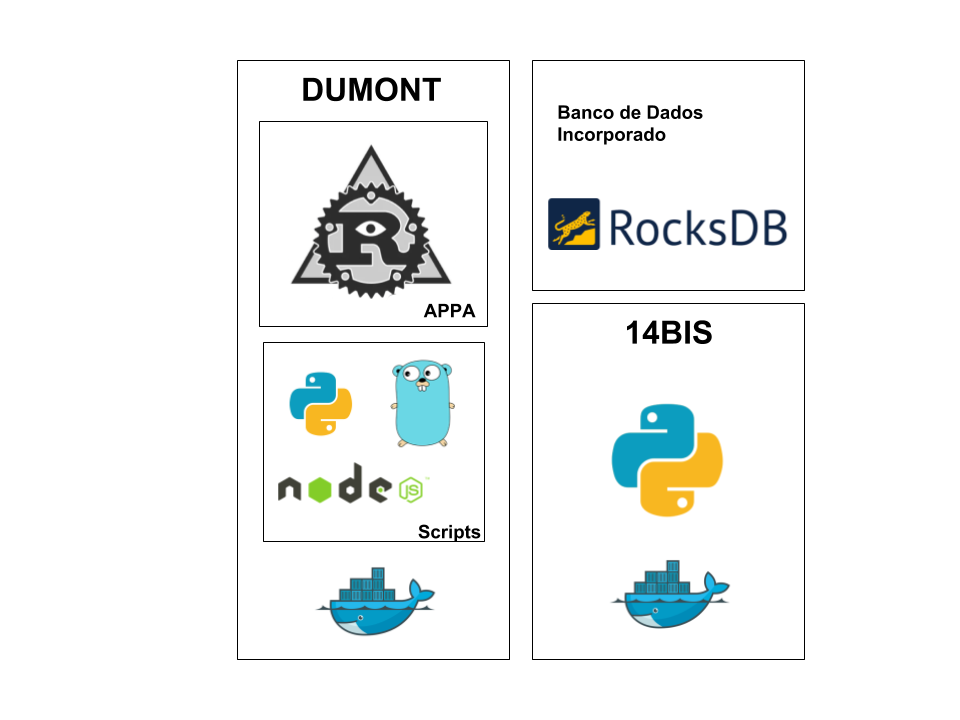
\includegraphics[width=1\textwidth]{imagens/tecnologias.png}
    \caption{Desenho apresentando os núcleos do projeto}
    \label{fig:tecnologias}
\end{figure}

Existem basicamente 5 técnologias que estão sendo utilizadas nesse projeto:
\begin{itemize}
 \item Python: É a linguagem atual mais utilizada no mundo de Aprendizado de Máquina, sua simplicidade ja á torna simples de usar, porém, a quantidade de materiais, bibliotecas e artigos sobre PLN e Aprendizado de Máquina á tornam a principal linguagem nesse projeto.
 \item Node/Javascript: Node é o interpretador que permite com que seja possivel executar o Javascript (linguagem originalmente de navegar no servidor). A linguagem tem um grande ganho com integrações e será utilizada para consumir recursos vindos de APIs.
 \item Go: Linguagem fortemente e estaticamente tipada, que fornecesse um poder de processamento equivalente a da linguagem C, entretando, muito mais simples de escrever e manter código, será utilizado para scripts onde serão necessário processamento de muitos dados.
 \item MongoDB: O Mongo é um banco não relacionado, em resumo, um grande banco de documentos indexados por atributos especificos, fornece um grande poder de leitura alem do fato de não ser prezo a estruturas pré-definidas como banco relacionais (isso facilita para que sejam inseridos novos dados futuramente sem grandes custos).
 \item Docker: Docker é uma ferramenta para infra-estrutura, será utilizado para rodar a aplicação em containers e facilitar o \textit{deploy}\footnote{Vindo do termo em inglês "lançar" é utilizado para o ato de colocar uma aplicação em ambiente de produção}.
\end{itemize}

Uma vez obtido conhecimento sobre os núcleos do projeto e suas técnologias, é possível idealizar o fluxo completo e interação entre elas. Se observar a Figura \ref{fig:tcc_caso_de_uso}, notara que o Dumont ira utilizar da API do twitter para coletar dados públicos, posteriormente esses dados serão processados e mutacionados a fim de gerar uma base de dados, por final essa base dados será salva em um banco de dados.

\begin{figure}
    \centering
    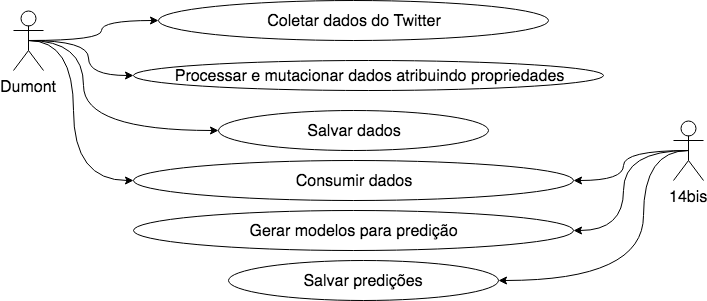
\includegraphics[width=.6\textwidth]{imagens/tcc_caso_de_uso.png}
    \caption{Diagrama de caso de uso do sistema}
    \label{fig:tcc_caso_de_uso}
\end{figure}

Revisando e reafirmando tudo o que foi dissertado até então, nosso objetivo é gerar uma base de conhecimento, aplica-la a uma aprendizagem supervisionada e em seguida aplicar esse dado a uma não supervisionada. Logo a primeira etapa é adquirir o \textit{dataset} que será utilizado.

\section{Coletando Base de Dados}
A primeira etapa do processo inclui coletar dados para que, posteriormente, seja possível mineirar atributos dentro deles. O coletor é algo simples, basicamente um script que roda de tempos em tempos baseado na configuração apresentada. Foi desenvolvida uma função responsável por coletar em tempo real tweets em uma determinada área e que em seu corpo tivesse uma ou mais palavras chaves. Com isso é possível pesquisar um usuário e seus últimos 200 tweets.

De todos os modelos previamente explicados, os utilizados dentro do coletor são os de \textit{user} e \textit{tweet}. Eles podem ser encontrados dentro de \textit{dumont/collector/schemas}. Antes do dado ser salvo é possível notar a criação de um objeto partindo do atributo de texto referente ao tweet. Um dos problemas durante a mineração de dados é o uso de \textit{emojis} em textos. Sabendo que \textit{emojis} podem expressar sentimentos, armazenar e tratar esses dados poderia ser relevante na hora de confirmar o sentimento em frases, durante esse processo a lógica para localizar e extrair esses elementos foi abstraida para uma biblioteca chamada \textit{Emojinator}\footnote{https://github.com/getdumont/emojinator}. Além do texto tratado, também será obtida informações do \textit{emojis} utilizados no meio do texto.

Para ativar o coletor foi criado um CLI\footnote{CLI é abreviatura para \textit{Command Line Interface}, em outras palavras, uma interface que permite executar códigos direto do terminal}. Antes de rodar o comando é necessário configurar o projeto conforme o \autoref{app:configuracoes}. Após terminar a configuração rode o comando \textit{docker-compose up collector}, logo que finalizar a coleta vai preencher seu MongoDB com os dados necessários para as próximas etapas. Durante essa pesquisa o comando foi rodado diversas vezes em um periodo de tempo, para criar uma base inicial. Vale lembrar que a idéia final se consiste em um mapeando periódico de perfis, porém nesse momento o coletor foi feito unicamente para juntar um aglomerado de dados indiferente de seus perfis.

No primeiro momento que o coletor foi rodado na pesquisa, foram coletados um total de 68583 tweets distribuídos entre 419 perfis, gerando uma média de aproximadamente 163 tweets por usuário. A massa de dados é bem ampla e achar uma amostra que suprisse as necessidades poderia ser algo complexo. Para isso o enfoque inicial é localizar uma amostra com os perfis que contem a maior massa de tweets negativos, entretanto, isso não é possível sem idealizar uma segunda parte do processo, no caso o pré-processamento e a mineração.

